Particle accelerators were first developed in the early 20th century as a tool for high-energy physics research. By increasing particles' energy they allow us to investigate the subatomic structure of the world and to study the properties of the elementary particles and the fundamental forces. On a basic level, accelerators increase the energy of charged particles using electromagnetic fields. Through the years significant technological progress has been achieved resulting in higher energies and optimising the performance of the machines. Additionally, various types of accelerators have been developed (synchrotrons, colliders etc) using different types of particles (hadrons or leptons) and its use was also expanded in other fields such as medicine and industrial research. 
% Brief history of particle accelerators: https://cds.cern.ch/record/261062/files/p1_2.pdf
% Summary for accelerators: https://www.energy.gov/articles/how-particle-accelerators-work#:~:text=There%20are%20two%20primary%20roles,charged%20particles%20for%20medical%20treatment.



\section{The CERN accelerator complex}

CERN (European Organisation of Nuclear Research), located on the Franco-Swiss border near Geneva, is at the forefront of the accelerator physics research as it operates an extensive network of accelerators, illustrated in Fig.~\ref{fig:cern_accelerator_complex}, including the well-known Large Hadron Collider (LHC)~\cite{Brüning:782076}.

LHC is a circular machine, 27\, km long, built about 100\,m underground and is currently the largest and most powerful accelerator. It accelerates and collides two counter-rotating beams at the four main experiments which are located around the LHC ring, namely ATLAS, CMS, ALICE and LHCb. The highlight of CERN and of the LHC operation up to now was the discovery of the Higgs boson in 2012 from ATLAS~\cite{ATLAS_Higgs} and CMS~\cite{CMS_Higgs}, from proton collisions at 3.5\,TeV (center-of-mass energy of 7\,TeV), which was a milestone for the standard model. % Importance of higgs discovery: https://home.cern/resources/faqs/cern-and-higgs-boson

The beams used by the LHC, are produced and gradually accelerated by the injector chain which is basically a sequency of smaller machines boosting subsequently the energy of the beam. In particular, Linac4 (replaced Linac2 in 2020) accelerates the protons up to 160\,MeV, the Proton Synchrotron Booster (PSB) up to 2\,GeV, the Proton Synchrotron (PS) up to 26\,GeV and the the Super Proton Synchrotron (SPS) up to 450\,GeV. Finally, the protons are injected in the LHC machine where they are accelerated up to the collision energy of at 6.5\,TeV (center-of-mass energy of 13\,TeV). It should be noted, that LHC delivered colissions with center-of-mass energy of 7\,TeV during Run 1 (2010-2013) which was increased to 13\,TeV for the Run 2 (2015-2018) and for Run 3 (2020-present). 
% actually from april 2012 till the end of run 1 it deleveled 8 TeV. 

\begin{figure}[!h] %https://cds.cern.ch/images/CERN-GRAPHICS-2022-001-1
    \centering         
    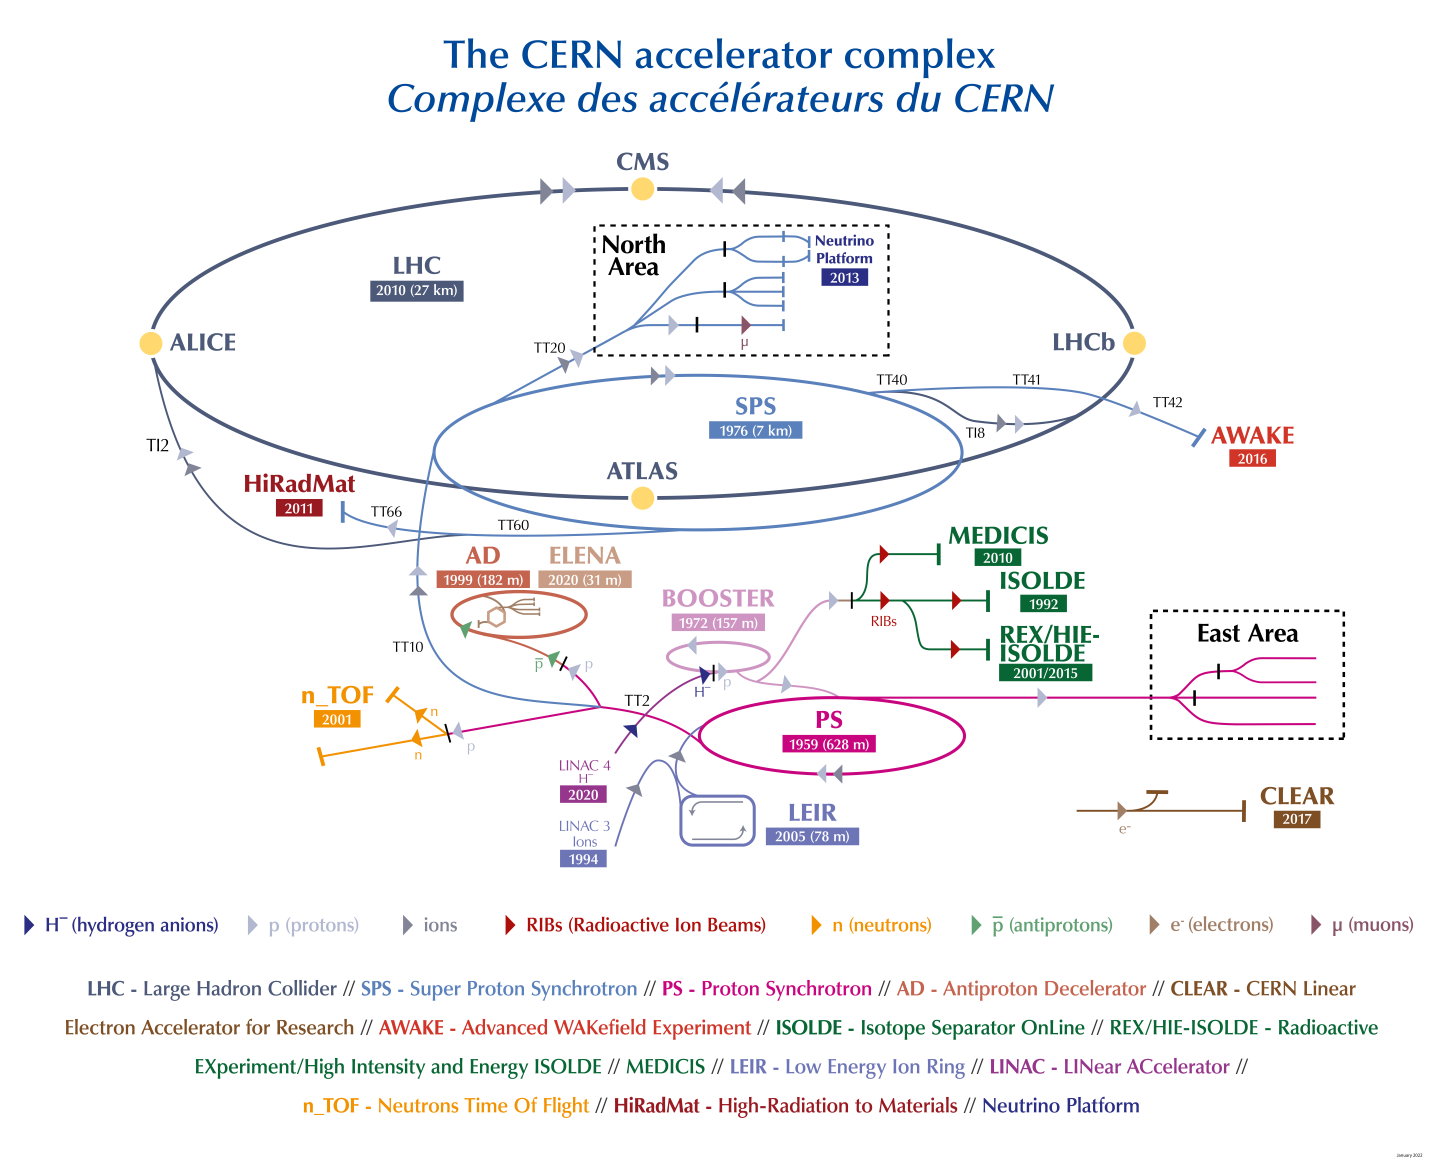
\includegraphics[width=1\textwidth]{images/introduction/cern_accelerator_complex.png}
        \caption{Schematic view of the CERN accelerator complex. The different colors correspond to the different machines. The year of commissioning and the type of particles used in each one of them are also indicated along with the circumference for the circular machines. The image is a courtesy of CERN.}
        \label{fig:cern_accelerator_complex}
 \end{figure}

 It is worth mentioning that not only protons but also led ions are accelerated in the LHC, starting their journey from Linac3 and LEIR and then following the same route with proton beams.


 Last, the accelerators in the injector chain not only prepare the beam for the LHC but also provide beams to various other facilities and experiments at lower energies. Examples are the Anti-proton Decelerator (AD) which studies the antimatter, the Online Isotope Mass Separator (ISOLDE) which studies the properties of the atomic nuclei using radioactive beams, and the Advanced Proton Driven Plasma Wakefield Acceleration Experiment (AWAKE) which investigates the particles' acceleration by proton-driven plasma wakefield.

 \subsection{The CERN Super Proton Synchrotron}
 % sps history: https://be-dep-op-sps.web.cern.ch/history
 The majority of the research described in this thesis was conducted for the Super Proton Synchrotron (SPS). Thus, some additional information about this machine is provided here. The SPS (shown with light blue color in Fig.~\ref{fig:cern_accelerator_complex}) was switched on in 1967 and has a circumference of 6.9\,km. It used to operate as a proton-antiproton collider ($\mathrm{Sp\bar{p}S}$) and later on as an injector for the Large Electron Positron collider (LEP) while it also provided beams for fixed-target experiments (e.g. in the North Area). Even though the SPS can accelerate various particle types (protons, antiprotons, electrons, and heavy ions) the following information will concern its operation with proton beams which is the topic of the research presented in this thesis.

 Currently, the SPS is the second biggest accelerator at CERN and it can accelerate protons in from 26\,GeV up to 450\,GeV. Due to its past use as a collider, it can also operate as a storage ring. This operational mode is called "coast" and was used for the majority of the experimental studies presented in this thesis. During coast, the bunches circulate in the machine for long periods at constant energy. The highest energy at which SPS can operate in coast is 270\,GeV. 

 %After that they are injected in the LHC. Hoewever, as it used to be a collider it can operate as a storage ring, it is called coast (des ti exeis grapsei.) and will be used for the studies in this thesis.
 



\section{High-Luminosity LHC project and Crab Cavities}
%LHC is the flagship of the CERN accelerator complex and is the at the cutting edge of the accelerator and high energy physics research with almost ten thousand scientists working for and with it. In order to extend its discovery potential LHC will undergo a major upgrade in the coming years. 
% Hl-lhc book: p.2 hl-lhc is the top priority of the european strategy of particle physics. 
High-Luminosity LHC (HL-LHC)~\cite{HL_LHC_yellow_report, Brning2015} is the upgrade of the LHC machine which will extend its potential for discoveries. In particular, it aims to increase its instantaneous luminosity by a factor of 5 beyond the current values and the integrated luminosity by a factor of 10. 

The luminosity, along with the energy, is a key parameter defining the performance of a collider as it is a measure of the collisions rate. The instantaneous luminosity is expressed as~\cite{luminosity}:

\begin{equation}\label{eq:luminosity_inst}
    \mathcal{L} = \frac{n_b f_\mathrm{rev}N_1 N_2}{4 \pi \sigma_x \sigma_y} \frac{1}{\sqrt{1+(\frac{\sigma_z}{\sigma_\mathrm{xing}} \frac{\theta_c}{2})^2}},
\end{equation}

where $\frev$ is the revolution freuency of the machine, $n_b$ is the number of colliding bunch pairs, $N_{1,2}$ is the bunch intensity, $\sigma_{x,y}$ is the transverse beam size at the interaction point, $\sigma_z$ the rms bunch length, $\sigma_{\mathrm{xing}}$ the transverse beam size in the crossing plane and $\theta_c$ is the full crossing angle between the colliding beams.

The integrated luminosity, is the one that ultimately defines the performance of the machine as it provides the total number of recorderd events. It depends both on the instantaneous luminosty and on the machine availability. The integrated luminosity, is expressed as~\cite{HL_LHC_yellow_report}:
\begin{equation}\label{eq:integrated_luminosity}
    \mathcal{L}_I \equiv \int_{\Delta t} \mathcal{L} dt,
\end{equation}

where $\mathcal{L}$ the instantaneous luminosity as defined in Eq.~\eqref{eq:luminosity_inst}.
% for more details and specific values check sofias thesis.



\normalsize{\textbf{Crab Cavities}}\\
HL-LHC will employ a number of innovative technologies to achieve its luminosity goals. Crab Cavity (CCs) is one of the key componenets of the project as they will be employed to restore the luminosity reduction caused by the crossing angle, $\theta_c$ (see Eq.~\eqref{eq:luminosity_inst}).



Why do we need hl-lhc.
%https://slideplayer.com/slide/8611970/ slide 3

extend/push the discovery potential (Sofia.)

HL-lHC a major upgrade, priority of the european strategy





High-Luminosity LHC (HL-LHC) project~\cite{HL-LHC} is the upgrade of the LHC machine, which aims to increase its integrated luminosity production by a factor of 10 beyond the current operational values.


Crab cavities (will be denoted as $\CC$ in this thesis) is one of the key components of the High Luminosity LHC





\section{Motivation, objectives and thesis outline}

\textbf{Probably put to abstract}\\
In 2018, two prototype Crab Cavities ($\CC$s) were installed in the SPS to be tested for the first time with proton beams. A series of dedicated machine developemnt studies was carried out in order to validate their working principle and answer various beam dynamic questions. One of the operational issues that needed to be addressed concerned the expected emittance growth due to noise in their RF system, which is the main subject this thesis.  As mentioned in chapter~\ref{Ch:CC_noise_theory} a theoretical model had already been developed and validated by trackig simulations~\cite{PhysRevSTAB.18.101001}. 
As a part of the first experiemental campaign with $\CC$s in SPS a dedicated experiment was conducted to benchmark these models with experimental data and confirm the analytical predictions. The objective of this chapter is to provide an overview of the machine setup for the $\CC$ experiements and introduce the instruments and methods used for measuring the beam parameters of interest for the emittance growth studies.

\section{General parameters of the studies}
% Maybe this should be mentioned at the end of project objectives and thesis outline.
% The following paragraphs are taken from the APR Ch.1.3 
\subsection{SPS optics}\label{subsec:SPS_optics_model}
 The studies presented in this thesis were performed for the nominal SPS optics for the LHC filling which are called Q26 optics as the higher integer part of the tune in both planes is 26. 

 \normalsize{\textbf{SPS nominal model}\\
 The model for the Q26 optics can be found in the official CERN repository~\cite{SPS_optics_repo} and will be referred to as the nominal SPS model in this thesis. The values of the optics parameters in what follows correspond to the model values unless stated otherwise.

 \normalsize{\textbf{SPS non-linear model}\\
The nominal SPS model includes only the nonlinear fields produced by the chromatic sextupoles. However, one of the most important sources of non-linearities in SPS are the odd multipole components of its main dipole magnets. For some of the studies presented in this thesis their impact on the beam dynamics must be studied and therefore they should be included in the nominal model. 

% APR Chapter 3.1
The multipole error of the SPS main dipoles are unfortunately not available from magnetic measurements. On this ground a non-linear optics model of the SPS has been established with beam-based measurements of the chromatic detuning over a range of momentum deviation~\cite{Carlà:2664976, Alekou:2640326}.  The optics model was obtained by assigning systematic multipole components to the main lattice magnets, in the nominal model of SPS, in order to reproduce the tune variation with themomentum deviation as it was measured in the real machine. The calculations were performed with MAD-X [].

The values of the multipole components up to seventh order obtained from this method are given in Table~\ref{tab:sps_mult_270GeV} where, ($b_3^A, b_3^B$) ($b_5^A, b_5^B$) and ($b_7^A, b_7^B$) stand for the sextupolar, decapolar and decatetrapolar mutipoles respectively. Note that different values have been obtained foreach of the two different kinds of SPS main dipoles (MBA and MBB) which are marked withthe indices A and B respectively.

\begin{table}[ht] % table take from the APR
    \caption{Multipole errors from SPS non-linear model, at 270\,GeV.} % title of Table
    \centering % used for centering table
    \begin{tabular}{c c c c} % centered columns (4 columns)
    \hline\hline %inserts double horizontal lines
    Multipole & Value  \\ [0.5ex] % inserts table
    %heading
    \hline  % inserts single horizontal line
    $b_3^A, b_3^B$ & 8.1 $\times 10^{-4}$\,$\mathrm{m^{-2}}$, 1.1 $\times 10^{-3}$\,$\mathrm{m^{-2}}$\\ 
    $b_5^A, b_5^B$ & 9.2\,$\mathrm{m^{-4}}$, $-$10\,$\mathrm{m^{-4}}$ \\
    $b_7^A, b_7^B$ & 1.3 $\times 10^{5}$\,$\mathrm{m^{-6}}$, 1.4 $\times 10^{5}$\,$\mathrm{m^{-6}}$\\ [1ex] % [1ex] adds vertical space
    \hline %inserts single line
    \end{tabular}
    \label{tab:sps_mult_270GeV} % is used to refer this table in the text
    \end{table}


\textbf{random multiple errros? } Like in APR.Ch.3.2.2.